\documentclass[oneside]{article}
\setlength{\oddsidemargin}{0.25 in}
\setlength{\evensidemargin}{-0.25 in}
\setlength{\topmargin}{-0.6 in}
\setlength{\textwidth}{6.5 in}
\setlength{\textheight}{8.5 in}
\setlength{\headsep}{0.75 in}
\setlength{\parindent}{0 in}
\setlength{\parskip}{0.1 in}
\usepackage{xcolor}
\usepackage{graphicx}
\usepackage{subcaption}
\usepackage{mwe}
\usepackage{dirtytalk}
\usepackage{amsmath,amsfonts}
\usepackage{makecell} 
\usepackage{algorithm,algcompatible}
\usepackage{float}
\usepackage[a4paper,bindingoffset=0.2in,%
            left=0.5in,right=0.5in,top=0.5in,bottom=0.5in,%
            footskip=.25in]{geometry}

\newcounter{lecnum}
\renewcommand{\thepage}{\arabic{page}}
\renewcommand{\thesection}{\arabic{section}}
\renewcommand{\theequation}{\arabic{equation}}
\renewcommand{\thefigure}{\arabic{figure}}
\renewcommand{\thetable}{\arabic{table}}
\usepackage{listings}
\usepackage{kotex}
\lstdefinelanguage[RISC-V]{Assembler}
{
  alsoletter={.}, % allow dots in keywords
  alsodigit={0x}, % hex numbers are numbers too!
  morekeywords=[1]{ % instructions
    lb, lh, lw, lbu, lhu,
    sb, sh, sw,
    sll, slli, srl, srli, sra, srai,
    add, addi, sub, lui, auipc,
    xor, xori, or, ori, and, andi,
    slt, slti, sltu, sltiu,
    beq, bne, blt, bge, bltu, bgeu,
    j, jr, jal, jalr, ret,
    scall, break, nop
  },
  morekeywords=[2]{ % sections of our code and other directives
    .align, .ascii, .asciiz, .byte, .data, .double, .extern,
    .float, .globl, .half, .kdata, .ktext, .set, .space, .text, .word
  },
  morekeywords=[3]{ % registers
    zero, ra, sp, gp, tp, s0, fp,
    t0, t1, t2, t3, t4, t5, t6,
    s1, s2, s3, s4, s5, s6, s7, s8, s9, s10, s11,
    a0, a1, a2, a3, a4, a5, a6, a7,
    ft0, ft1, ft2, ft3, ft4, ft5, ft6, ft7,
    fs0, fs1, fs2, fs3, fs4, fs5, fs6, fs7, fs8, fs9, fs10, fs11,
    fa0, fa1, fa2, fa3, fa4, fa5, fa6, fa7
  },
  morecomment=[l]{;},   % mark ; as line comment start
  morecomment=[l]{\#},  % as well as # (even though it is unconventional)
  morestring=[b]",      % mark " as string start/end
  morestring=[b]'       % also mark ' as string start/end
}

% usage example:

% define some basic colors
\definecolor{mauve}{rgb}{0.58,0,0.82}

\lstset{
  % listings sonderzeichen (for german weirdness)
  literate={ö}{{\"o}}1
           {ä}{{\"a}}1
           {ü}{{\"u}}1,
  basicstyle=\normalsize\ttfamily,                    % very small code
  breaklines=true,                              % break long lines
  commentstyle=\itshape\color{green!50!black},  % comments are green
  keywordstyle=[1]\color{blue!80!black},        % instructions are blue
  keywordstyle=[2]\color{orange!80!black},      % sections/other directives are orange
  keywordstyle=[3]\color{red!50!black},         % registers are red
  stringstyle=\color{mauve},                    % strings are from the telekom
  identifierstyle=\color{teal},                 % user declared addresses are teal
  frame=l,                                      % black line on the left side of code
  language=[RISC-V]Assembler,                   % all code is RISC-V
  tabsize=4,                                    % indent tabs with 4 spaces
  showstringspaces=false                        % do not replace spaces with weird underlines
}

\newcommand{\lecture}[4]{
   %\pagestyle{myheadings}
   %\thispagestyle{plain}
   \newpage
   \setcounter{page}{#3}
   \noindent
   \begin{center}
   \framebox{
        \vbox{\vspace{2mm}
        \hbox to 6.28in { {\bf 2023 ASIC Design Mid-Term project
	       \hfill 2023.11.06.} }
        \vspace{4mm}
        \hbox to 6.28in { {\Large \hfill \textbf{#2} \hfill} }
        \vspace{2mm}
        \hbox to 6.28in { { Name: \textbf{#1} \hfill } }
        \vspace{2mm}}
   }
   \end{center}
}

\renewcommand{\cite}[1]{[#1]}
\def\beginrefs{\begin{list}%
        {[\arabic{equation}]}{\usecounter{equation}
         \setlength{\leftmargin}{2.0truecm}\setlength{\labelsep}{0.4truecm}%
         \setlength{\labelwidth}{1.6truecm}}}
\def\endrefs{\end{list}}
\def\bibentry#1{\item[\hbox{[#1]}]}

\newcommand{\fig}[3]{
			\vspace{#2}
			\begin{center}
			Figure \thelecnum.#1:~#3
			\end{center}}
\newtheorem{theorem}{Theorem}[lecnum]
\newtheorem{lemma}[theorem]{Lemma}
\newtheorem{proposition}[theorem]{Proposition}
\newtheorem{claim}[theorem]{Claim}
\newtheorem{corollary}[theorem]{Corollary}
\newtheorem{definition}[theorem]{Definition}
\newenvironment{proof}{{\bf Proof:}}{\hfill\rule{2mm}{2mm}}

\newcommand\E{\mathbb{E}}

\begin{document}
\lecture{Jinmo Ahn}{5-stage Risc-V Processor Design}{1}{2017160111}

\section{Schematic and Explain my design in detail}
\subsection{Overall CPU design}
\begin{figure}[h]
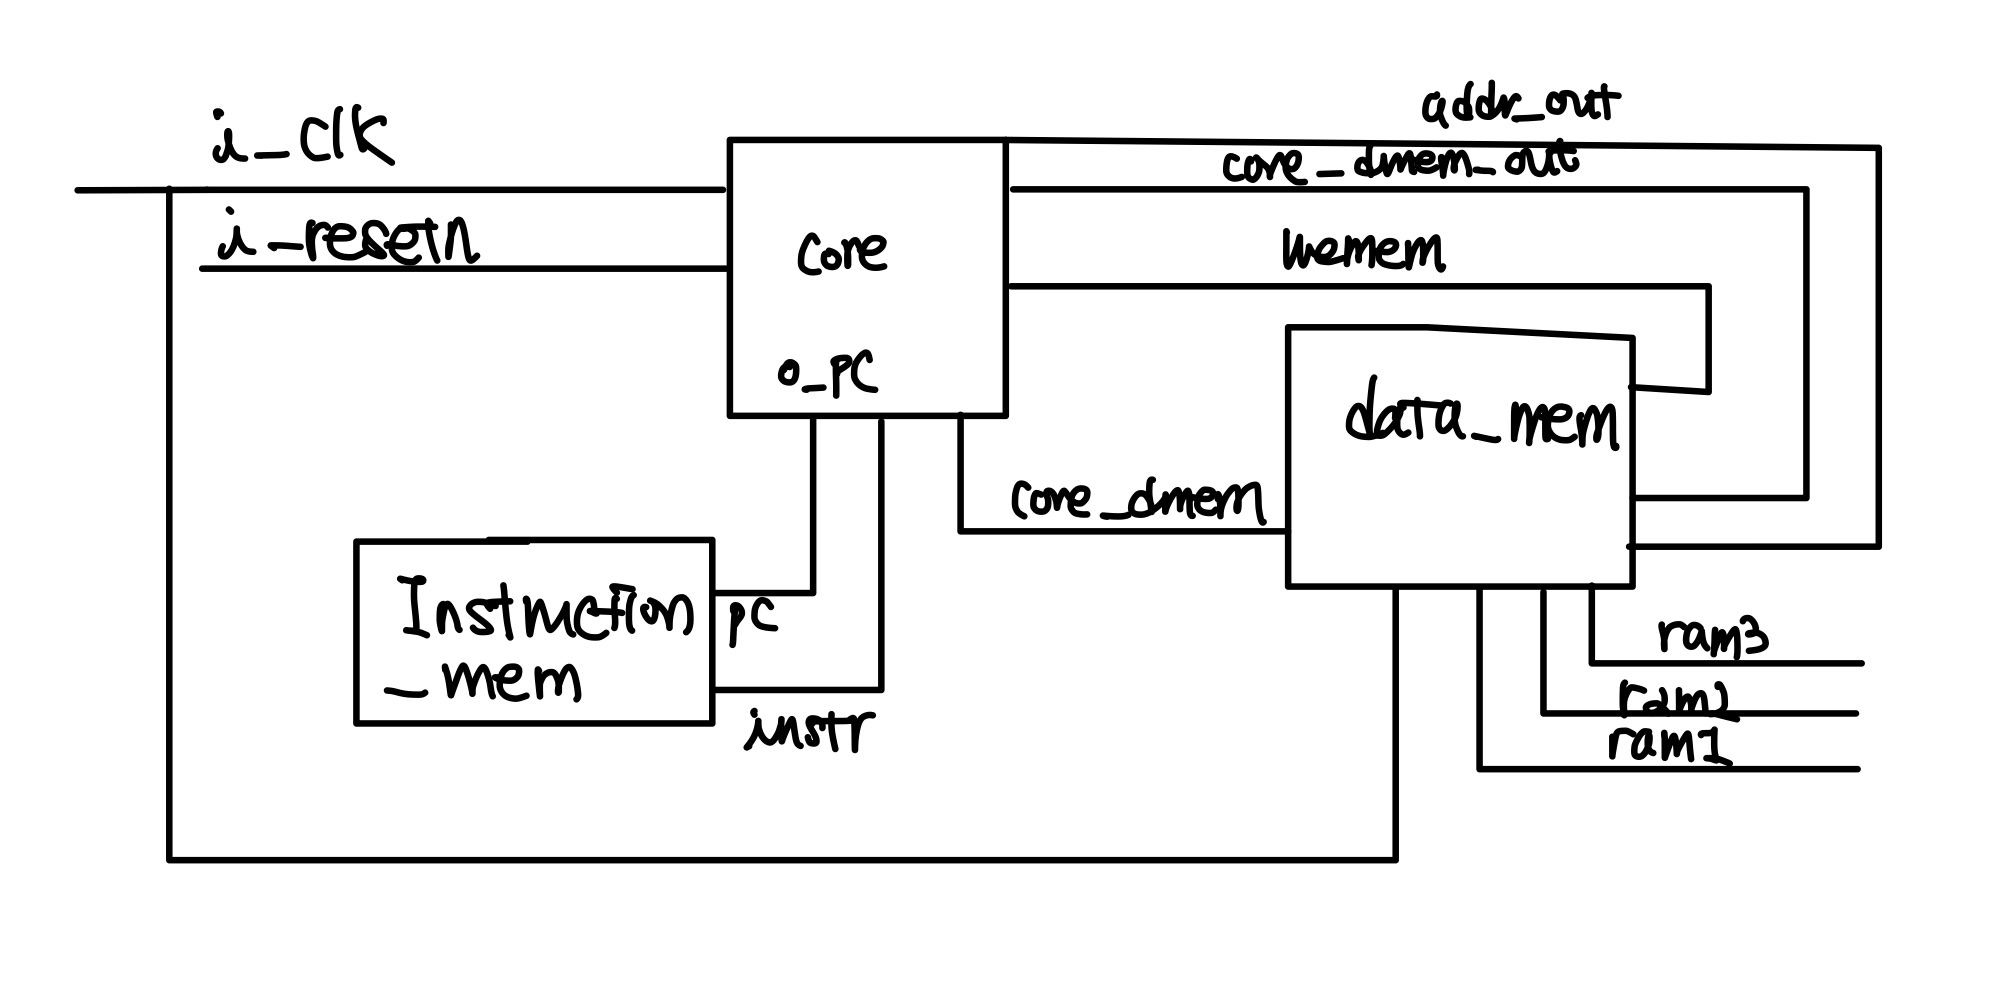
\includegraphics[width=12cm]{Image-1.jpg} 
\centering
\caption{Overall Design}
\end{figure}
Overall Schematic은 위와 같다. 여기서, Core part는 당연히 I/O signal을 Processing하는 part이고, 우리가 구현하고자 하는 Havard Architecture에 맞추어 D/I mem을 구분하였다. Imem의 경우 주어진 구현에 맞추어, $\textdollar$readmemh 의 구문을 아래처럼 넣어주었다.

\begin{center}
\begin{tabular}{c}
\begin{lstlisting}[language=Verilog]
$readmemh ("test_program2.txt",rom);
\end{lstlisting}
\end{tabular}
\end{center}



다음은 data-mem이다. 사실 우리가 RTL Verification 만으로는 실제 RAM에 접근하기 어려워, 이를 Flip-Flop으로 설계하였다. 또한 여기서 ram1 ,ram2 ,ram3는 [31:0] ram [0:31]중 ram[0], ram[1], ram[2]에 wire한 내용으로, 내부에 저장이 잘 되었는지 확인하기 위해 바깥으로 빼서 놓았다. 따라서 향후 저장 시에, 주소를 0,1,2 에만 저장하는 것을 볼 수 있을 것이다. 이를 직접적으로 코드로 확인하면 아래와 같다.  (ex. sw x18, 0(x0) /  In Risc V, x0 is hardly wired to zero)\\ 
\begin{center}
\begin{tabular}{c}
\begin{lstlisting}[language=Verilog]
   reg [31:0] ram [0:31];
    assign ram1 = ram[0];
    assign ram2 = ram[1];
    assign ram3 = ram[2];
    
    always @(posedge i_clk)
    begin
        if(we)
         ram[i_addr[4:0]] = i_data;
    end
    
    integer i;
    initial
    begin
        for(i=0;i<32;i=i+1)
            ram[i] = 0;
    end
\end{lstlisting}
\end{tabular}
\end{center}
\begin{center}
Data memory Verilog Source code
\end{center}
마지막으로 Core unit인데, 이는 아래에서 자세히 알아보도록 하자.

\subsection{Core design}
Core의 component는 우리가 일반적으로 아는 RISC 계열 CPU와 동일하다. PC register와, 각종 signal에 따라 output 값을 바꿔주는 Mux, Control unit이 있다. 또한 CPU의 SRAM과 동일한 역할을 하는 Register file이 존재한다. 해당 Design에서 CLA (carry look-ahead adder)를 사용하여 더욱 빠른 Computation을 하도록 하였으며, Control Hazard를 약간이라도 개선하기 위한 Comparator unit과, Static Branch non-taken mode를 사용하였다. 사실 Dynamic branch prediction과 Static Branch Prediction이 큰 차이가 나지 않는다는 것에 기인해서 앞선 mode를 사용하였다. 하지만, 여전히 1cycle의 Stall을 사용하여야 한다. (Double pumping까지 이용한다면, 가능할 수도 있으리라 생각한다.) 또한 각각 Control signal, Data 등에 맞추어 Pipeline register를 apply해주었다.

\section{Validation Scenarios}

\subsection{Scenario 1 - Tagetting a Control Hazard}

먼저, c언어로, 변수 초기화를 진행하고, ALU operation을 진행한 후, if문+함수를 통해 프로시저 콜을 하고, 받은 value를 store하는 시나리오를 생각하자. 간단하게 Assembly로 생각하면 register에 0를 apply하고 간단한 ALU 이후 beq/bne로 분기를 한다. 이후, 해당 branch 내부에서 ALU를 진행한 후, 다시 Unconditional branch로 돌아온 후 store를 하면 된다.  (control Hazard에 Reaction)

\begin{center}
\textbf{1. C language Source code}
\end{center}
\begin{center}
\begin{tabular}{c}
\begin{lstlisting}[language=C]
int main (void){
        int a = 0;
        int b = 0;
        a = a +3;
        b = b +2;
            int c=0;
                if (a != b){ // bne instruction
                  c = jinmo(a,b); // add a,b
    }
    return c;
}

int jinmo (int a,int b){
    return a+b; // store value & unconditional branch
}
\end{lstlisting}
\end{tabular}
\end{center}

\begin{center}

\end{center}

\begin{center}
\textbf{2. Compile to Risc-V Assembly }
\end{center}

\begin{center}
\begin{tabular}{c}
\begin{lstlisting}[language={[RISC-V]Assembler}]
MAIN:

 0 : add x19, x0, x0  /// a=0
 4 : add x20, x0, x0  /// b = 0
 8 : addi x19, x19, 3 /// a = a+3
12 : addi x20, x20, 2  /// b = b+2
16 : add x18, x0, x0 ///c =0
20 : bne x19, x20, L1 /// if (a != b)
24 : sw x18, 0(x0) // store to ram1

EXIT:

L1:  
40 (Just In my instruction memory) : add x18 x19 x20
44 beq x0 x0 24 (Loop 24)

\end{lstlisting}
\end{tabular}
\end{center}

\begin{center}

\end{center}
\newpage

\begin{center}
\textbf{3. Change to machine language }\\
1.	000009B3\\
2.	00000A33\\
3.	00398993\\
4.	002A0A13\\
5.	00000E33\\
6.	013A1A63\\
7.	01202023\\
8.	00000063\\
9.	00000063\\
10.	00000063\\
11.	01498933\\
12.	FE0006E3\\
\end{center}

이때, (Branch destination = Pc + sign-ext(imm[12:1] , 0) 이므로, 앞에 6번째 instruction인 013A1A63은 +20, 12번째 instruction에서는 -20을 sign-extention을 수행해주었다.\\
위와 같은 Test bench를 돌려보자. 모듈의 설명은 앞에서 진행했으므로, 생략한다. 따라서 txt file에 위의 instruction을 그대로 얹어주고, 총 cycle은 20사이클로 설정한 후, testbench를 돌리고 필요한 정보만 사진으로 캡처하면, 
\begin{figure}[h]
    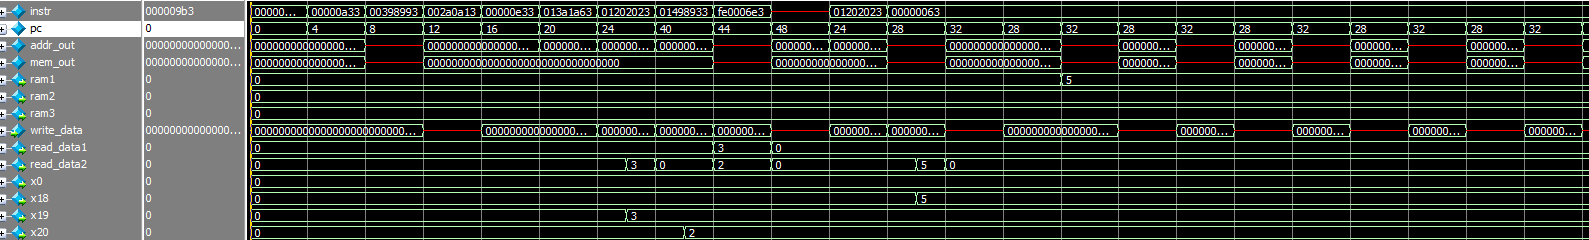
\includegraphics[width = 18cm]{Asic_s1.png}
    \centering
    \caption{S-1 Testbench}
\end{figure}
위와 같이, 우리가 생각한대로, PC shift를 하고, ALU를 진행한 후, ram1에 store하는 모습을 볼 수 있었다. (사진/tb file은 zip file로 같이 첨부하겠습니다.)

\subsection{Scenario 2 - Targetting a Data Hazard and verifying every instruction in PPT}
이번에는 C언어 없이 간단하게 assembly로만 생각하자. 먼저 어떠한 register에 하나의 값을 저장하고, 이후 그것을 ram에 저장, 이후 그것을 load하는 과정을 생각해보자. 그렇게 어렵지 않다. 이때, 
\\(Data Hazard를 check 하기위해, ALU operation을 연속으로 해보자.) 

\begin{center}
\textbf{1. Risc-V Assembly}
\end{center}

\begin{center}
\begin{tabular}{c}
\begin{lstlisting}[language={[RISC-V]Assembler}]
0 : add x19, x0, x0  
4 : add x20, x0, x0  
8 : addi x19, x19, 13 
12 : addi x20, x20, 5  
16 : sub x19,x19,x20
20 : add x19,x19,x20
24 : sw x19,0(x0)
28 : lw x18,0(x0)
32 : and x18, x18,x20
36 : or x17,x18,x19
40 : sll x16,x18,x19
44 : srl x16,x18,x19
48 : sra x16,x18,x19
52 : andi x16,x18,2
56 : ori x16, x18, 2
60 : sw x16,1(x0)
\end{lstlisting}
\end{tabular}
\end{center}

\begin{center}

\end{center}

\begin{center}
\textbf{2. Change to machine language }\\
1.	000009B3\\
2.	00000A33\\
3.	00D98993\\
4.	005A0A13\\
5.	414989B3\\
6.	014989B3\\
7.	01302023\\
8.	00002903\\
9.	01497933\\
10.	013968B3\\
11.	01391833\\
12.	01395833\\
13.	41395833\\
14.	00297813\\
15.	00296813\\
16.	010020A3

\end{center}
와 같고, 이에 대하여 test bench를 진행하면,
\begin{figure}[h]
    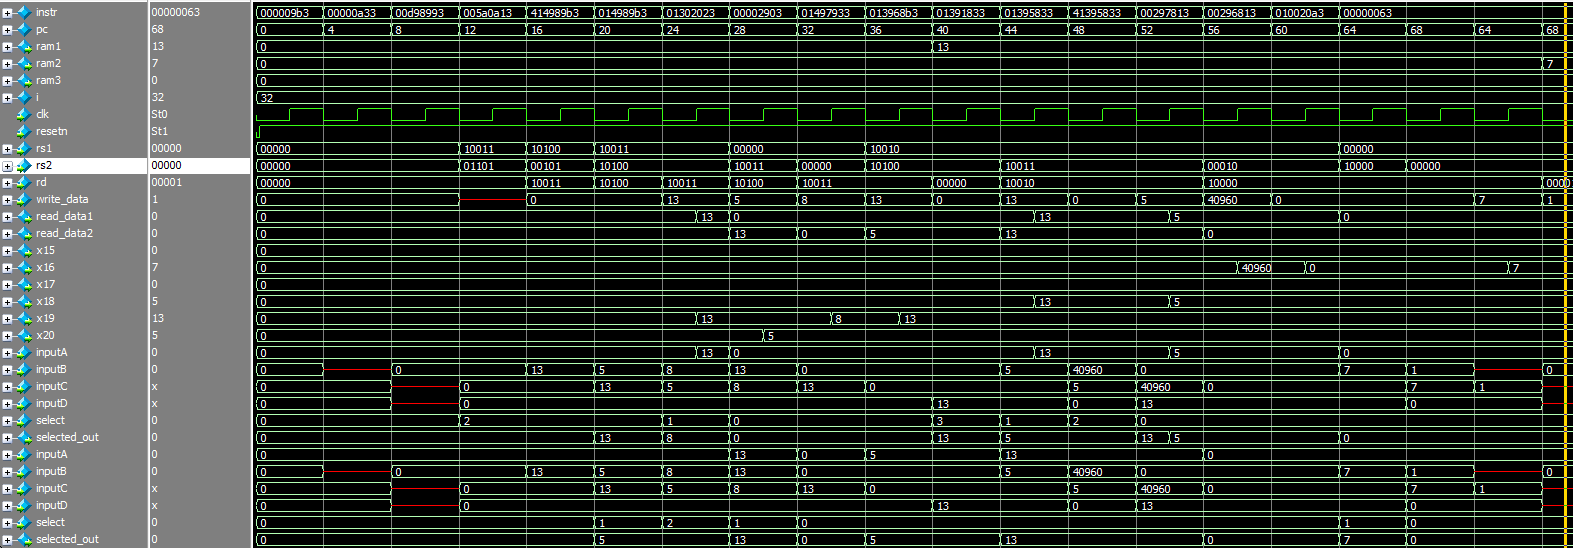
\includegraphics[width = 18cm]{ASIC_s2.png}
    \centering
    \caption{S-2 Testbench}
\end{figure}


와 같이 아주 정확하게 맞아 떨어지며, Forwarding unit이 정확하게 작동하여 위와 같이 CPU가 잘 동작하는 것을 확인할 수 있다.  또한 ram1, ram2에 정확히 저장이 된다. 이를 통해 모든 functionality와 data-Hazard 를 targeting한 processor에 대한 Validation이 완료되었다.

\section{Reference}
1. T.W.Seo (2021). Computer Architecture. Seoul, Korea: Hong pup science. \\
2. J.H. Kung (2023) Asic design Course materials

\end{document}

